\section{Thread Q Req-Spec}

Here we assemble notes about thread-Q requirements and specifications,
at a high level of abstraction.

A key concern is the maintenance of FIFO fairness.

\subsection{Scope}

We are working with scenarios involving semaphores
setup to be binary, using the priority inheritance protocol.

This requires the following semaphore attributes:
\begin{verbatim}
RTEMS_PRIORITY
RTEMS_BINARY_SEMAPHORE
RTEMS_INHERIT_PRIORITY
RTEMS_MULTIPROCESSOR_RESOURCE_SHARING
\end{verbatim}

This means we are using the MrsP protocol.

All notes below assume the above setup.

\subsection{Semaphore calls}

``
Call \verb"semaphore_obtain()" can return \verb"RTEMS_UNSATISFIED"
if there is a deadlock detected,
or it has been recursively called  by the same task.''

``Call \verb"semaphore_release()" can return \verb"RTEMS_INCORRECT_STATE"
if the calling task did did not respect
the expected acquisition and  release order.
Semaphores using this protocol must be released
in the opposite order with respect to the order in which they were obtained.''


MrsP requires a pre-scheduler ceiling priority for every mutex.
This is set using the \verb"priority_ceiling"  argument
of \verb"rtems_semaphore_create".

The above is from:
Bloom, Gedare; Sherrill, Joel; Hu, Tingting; Bertolotti, Ivan Cibrario.
Real-Time Systems Development with RTEMS and Multicore Processors
(Embedded Systems) (p. 245). CRC Press. Kindle Edition.

Bloom, G., Sherrill, J., Hu, T., \& Bertolotti, I.C. (2020).
Real-Time Systems Development with RTEMS and Multicore Processors (1st ed.).
CRC Press.
\verb"https://doi.org/10.1201/9781351255790"

\subsection{Priority Inheritance Protocol (PIP)}

``
The general idea of the priority inheritance protocol is to
dynamically increase the priority of a task
as soon as it is blocking some higher-priority tasks,
and run the  task at increased priority until it is no longer blocking them.
For example, as long as  a task (like $\tau$3 in Figure 8.1)
is blocking a higher-priority task (like $\tau$1 in the same  fgure)
it inherits its priority.''

``
In general,
as long as a task is blocking a set of higher-priority tasks,
it inherits the highest priority among them.''

Bloom, Gedare; Sherrill, Joel; Hu, Tingting; Bertolotti, Ivan Cibrario. Real-Time Systems Development with RTEMS and Multicore Processors (Embedded Systems) (p. 283). CRC Press. Kindle Edition.

We have:
\begin{itemize}
  \item task baseline vs. active priority
  \item scheduler uses active priority, with FCFS for same priority
  \item semaphore wait queues ordered by active priority.
\end{itemize}

\subsection{Priority Ceiling Protocol (PCP)}

This is PIP with the following added:
``
a task can be blocked not only because it attempted to acquire a busy semaphore,
as it happens for all kinds of mutual exclusion semaphore,
but also when acquiring a free semaphore could lead
a higher-priority task to be blocked more than once.''

Bloom, Gedare; Sherrill, Joel; Hu, Tingting; Bertolotti, Ivan Cibrario. Real-Time Systems Development with RTEMS and Multicore Processors (Embedded Systems) (p. 287). CRC Press. Kindle Edition.

We have that:
\begin{itemize}
  \item each semaphore has a fixed ceiling value,
  equal to the maximum initial priority of all tasks using the semaphore.
\end{itemize}

``
\begin{enumerate}
  \item
    When a task $\tau$ tries to acquire a semaphore,
    its active priority is checked against
    the ceiling of all currently busy semaphores,
    except the ones that $\tau$ has already acquired in the past and not released yet.
  \item
    If the active priority of $\tau$ is higher than all those ceilings,
    $\tau$ can proceed with the semaphore operation
    and possibly block if the semaphore is busy.
  \item
    Otherwise, $\tau$ is blocked until this condition becomes true,
    regardless of whether  the semaphore it is trying to acquire is busy or free.
    Afterwards, $\tau$ can proceed  with the semaphore operation.
\end{enumerate}
''

Bloom, Gedare; Sherrill, Joel; Hu, Tingting; Bertolotti, Ivan Cibrario. Real-Time Systems Development with RTEMS and Multicore Processors (Embedded Systems) (p. 288). CRC Press. Kindle Edition.

\subsection{Immediate Priority Ceiling Protocol (IPCP)}%
\footnote{
a.k.a. Priority Ceiling Emulation Protocol (PCEP)
}

Like IPCP, except that when a task acquires a semaphore its active priority
is immediately raised to the semaphore ceiling.

``
More formally,
at each instant
the active priority of a task is equal to the maximum
among its baseline priority
and the ceilings of all semaphores it has acquired and not released  yet so far.''

Bloom, Gedare; Sherrill, Joel; Hu, Tingting; Bertolotti, Ivan Cibrario. Real-Time Systems Development with RTEMS and Multicore Processors (Embedded Systems) (p. 288). CRC Press. Kindle Edition.

\textbf{Note: }
\textsf{Any change in task priority means updating the relevant queues}.

\subsection{Multiprocessor Resource Sharing Protocol (MrsP)}

This is derived from the priority ceiling protocols above.

``MrsP requires programmers to specify,
for each semaphore,
what is the priority of the highest-priority task
that can ever acquire that semaphore,
for each scheduler instance.
As a result,
each MrsP semaphore has multiple priority ceiling values,
one for each scheduler instance in the system.''

Bloom, Gedare; Sherrill, Joel; Hu, Tingting; Bertolotti, Ivan Cibrario. Real-Time Systems Development with RTEMS and Multicore Processors (Embedded Systems) (p. 456). CRC Press. Kindle Edition.

We note that:
\begin{itemize}
  \item
    ``When a task successfully acquires a semaphore,
      its priority is temporarily elevated
      to the ceiling priority of the semaphore
      for the scheduler instance the task is normally assigned to.
      In RTEMS,
      this scheduler instance is also called
      the home scheduler instance of the task.
      The priority elevation lasts until the task releases the semaphore.
      From this point of view,
      MrsP works in the same way as the immediate priority ceiling  protocol.''
  \item
    ``Tasks that are waiting to acquire a semaphore spin,
      that is,
      perform an active wait
      and remain running from the scheduler’s point of view,
      instead of waiting passively by
      moving to the blocked state of the task state diagram.
      Informally speaking,
      this prevents the spinning task from
      suffering further priority inversion-induced blocking
      after it eventually acquires the  semaphore,
      due to lower-priority tasks that might have been run
      and have  had their priority elevated by MrsP in the meantime.''
  \item
    ``In some cases,
      a helping protocol among scheduler instances
      may temporarily migrate a task from
      the set of cores it is normally assigned to,
      according to the partitioned or clustered scheduling approach,
      onto other cores.
      In the most basic case,
      this happens when the task is preempted
      by a higher priority task while it holds a semaphore,
      and on the other core there is a task waiting for the same semaphore.
      In other words,
      this also means that a task  may temporarily execute
      on cores that are not managed by its own home  scheduler instance,
      but belong to other scheduler instances
      where there is  at least another task that shares a semaphore with it.''
\end{itemize}

Bloom, Gedare; Sherrill, Joel; Hu, Tingting; Bertolotti, Ivan Cibrario. Real-Time Systems Development with RTEMS and Multicore Processors (Embedded Systems) (p. 457). CRC Press. Kindle Edition. ''

\subsection{MrsP on RTEMS}

A MrsP semaphore is built unlocked, with a given ceiling priority.
It's ceiling priority w.r.t. some scheduler may be different
and so may need tailoring.

Restrictions:
\begin{itemize}
  \item
    ``Tasks must release MrsP semaphores in the reverse order
      with respect to the sequence in which they were acquired,
      as it comes natural if critical regions are properly nested.
      Attempts to deviate from the prescribed order
      are detected and reported with
      the \verb"RTEMS_INCORRECT_STATE" status code upon semaphore release.''
  \item
    ``MrsP semaphores cannot be acquired recursively.
    Any attempt to do so results in
    the \verb"RTEMS_UNSATISFIED" status code being returned
    by \verb"rtems_semaphore_obtain".''
  \item
    ``Besides self-deadlocks
      that would result from recursive semaphore acquisition,
      the system also detects more complex kinds of deadlock
      that would be created by acquiring a semaphore.
      In this case, the \verb"rtems_semaphore_obtain" directive fails
      and returns the status code  \verb"RTEMS_UNSATISFIED".''
  \item
    ``Finally,
      but this is a restriction that does not concern only MrsP semaphores,
      an MrsP semaphore cannot be taken from an interrupt context
      or whenever thread dispatching is disabled.
      Any attempt to do so results in an internal RTEMS error
      or undefined behavior.''
\end{itemize}

Bloom, Gedare; Sherrill, Joel; Hu, Tingting; Bertolotti, Ivan Cibrario. Real-Time Systems Development with RTEMS and Multicore Processors (Embedded Systems) (p. 458). CRC Press. Kindle Edition. ''


\subsection{The MrsP Paper}

Notation: $\textrm{Quantity}_{\textrm{task}}^{\textrm{resource}}$.

Worst time execution of any task using resource $j$ is $c^j$.

No. of processors with tasks that access $r^j$ is $|map(G(r^j))|$.
$$
e_j = |map(G(r^j))|c^j
$$

\begin{quote}
``
Under MrsP we incorporate the property,
fundamental to the PCP/SRP protocol,
that once a task starts executing,
its resources will be logically available
–--
but the execution time required to use the resource is $e^j$ , not $c^j$ .
''
\end{quote}

From Section VI of MrsP paper (Burns and Wellings):


\begin{enumerate}
  \item
    All resources are assigned a set of ceiling priorities,
    one per processor
    (for those processors that have tasks that use the resource);
    for processor $p_k$ it is the maximum priority
    of all tasks allocated to $p_k$ that use the resource.
  \item
    An access request on any resource results
    in the priority of the task
    being immediately raised to the local ceiling for the resource.
  \item
    Accesses to a resource are dealt with in a FIFO order.
  \item
    While waiting to gain access to the resource,
    and while actually using the resource,
    the task continues to be active and executes
    (possible spinning)
    with priority equal to the local ceiling of the resource.
  \item
    Any task waiting to gain access to a resource
    must be capable of undertaking the associated computation
    on behalf of any other waiting task.
  \item
    This cooperating task must undertake
    the outstanding requests in the original FIFO order.
\end{enumerate}

\begin{quote}
``
The setting of the local ceiling for the resource
and the raising of the accessing task’s priority to the ceiling level
means that each processor implements a local PCP/SRP protocol.
''
\end{quote}

\begin{quote}
``
The key notion here is that a task is not spinning uselessly
while it is waiting to access the resource,
rather it is prepared to use its ‘wasted cycles’
to help other tasks make progress.
''
\end{quote}

\subsubsection{MrsP Properties}

\begin{description}
  \item [Lemma 1]
    ``
    At most one task per processor can be attempting
    to access any specific resource.
    ''
  \item [Lemma 2]
    ``
    The maximum length of the FIFO queue for resource $r^k$
    is $|map(G(r^k))|$.
    ''
  \item [Lemma 3]
    ``
    Each job can suffer at most a single local block,
    and this blocking will occur before it actually executes.
    ''
\end{description}

\subsubsection{Realising MrsP}

Task Migration:

\begin{quote}
``
If a task, $\tau_a$, is preempted whilst accessing a resource, $r^i$,
(by a higher priority local task)
then $\tau_a$ can migrate to any processor
on which a task is spinning
waiting to gain access to the same resource.
On this new processor $\tau_a$ is given the priority
one higher than the spinning task so that it preempts the spinning task.
''
\end{quote}

\begin{quote}
``
\dots
the requirement of the protocol:
that any spinning task can take over the resource access
on behalf of any other task is satisfied.
The spinning task just gives way to the migrating task
as the new task has a slightly higher priority.
In practice,
the supporting RTOS must be aware
that there is a separate priority associated
with each processor in the thread’s affinity set.
''
\end{quote}

\subsubsection{Prototype Implementation of MrsP}

Task t on processor p wants a lock on resource R:
\begin{verbatim}
Lock (R, t, p) ->
  raise priority of t to local ceiling of R
  Affinities(R) := Affinities(R) + p
  if already locked
    get current resource user R(t)
    Affinities(R(t)) := Affinities(R)
    obtain FIFO lock on R and spin
  else
    Affinities(t) := Affinities(R)
  end if
  set current lock holder to self
  raise priority of t by 1
  -- use R
\end{verbatim}

Releasing the lock on R held by task t, originally on processor p:
\begin{verbatim}
Unlock(R, t, p) ->
  Affinities(R) := Affinities(R) - p
  Release next task in FIFO queue (if there is one)
  Affinities(t) := p
  lower priority of t to its base value
\end{verbatim}


\subsection{The MrsP in RTEMS Thesis}

From:
Gomes. Ricardo,
``Analysis of MrsP Protocol in RTEMS Operating System'',
Licenciatura thesis,
Departmento de Engenharia Inform\'{a}tica, CISTER, Porto,
2019.

\begin{quotation}
``
In order to support the helping mechanism,
the RTEMS scheduler needs three indispensable operations,
“ask a scheduler node for help”,
“reconsider the help request of a scheduler node”
and “withdraw a scheduler node”
'' (pp34--35)
\end{quotation}

\begin{quotation}
``
MrsP is considered a mutex,
or binary semaphore,
since only one task at a time may obtain it,
granting mutual exclusion of resources.
Thus, being considered a resource sharing protocol.
Tasks access order to MrsP semaphores are dealt according to their priorities.
'' (p39)
\end{quotation}

\begin{quotation}
``
In this chapter,
the focus is the implementation of the most relevant operations
of a MrsP semaphore in RTEMS,
namely,
the creation of a semaphore,
changing its priority ceiling,
the resource release,
resource obtainment and,
finally,
the semaphore deletion.
`` (p41)
\end{quotation}

\begin{quotation}
``
MrsP is a priority ceiling-based resource sharing protocol,
that manages the access to a global resource using a FIFO queue.
In this way,
the structure that comprises a MrsP semaphore
must be composed of a global FIFO queue
to manage the access to the resource
and a set of priority ceiling values
used by each scheduler instance of the system,
these are responsible for managing the access to the FIFO queue locally.
'' (p41)
\end{quotation}


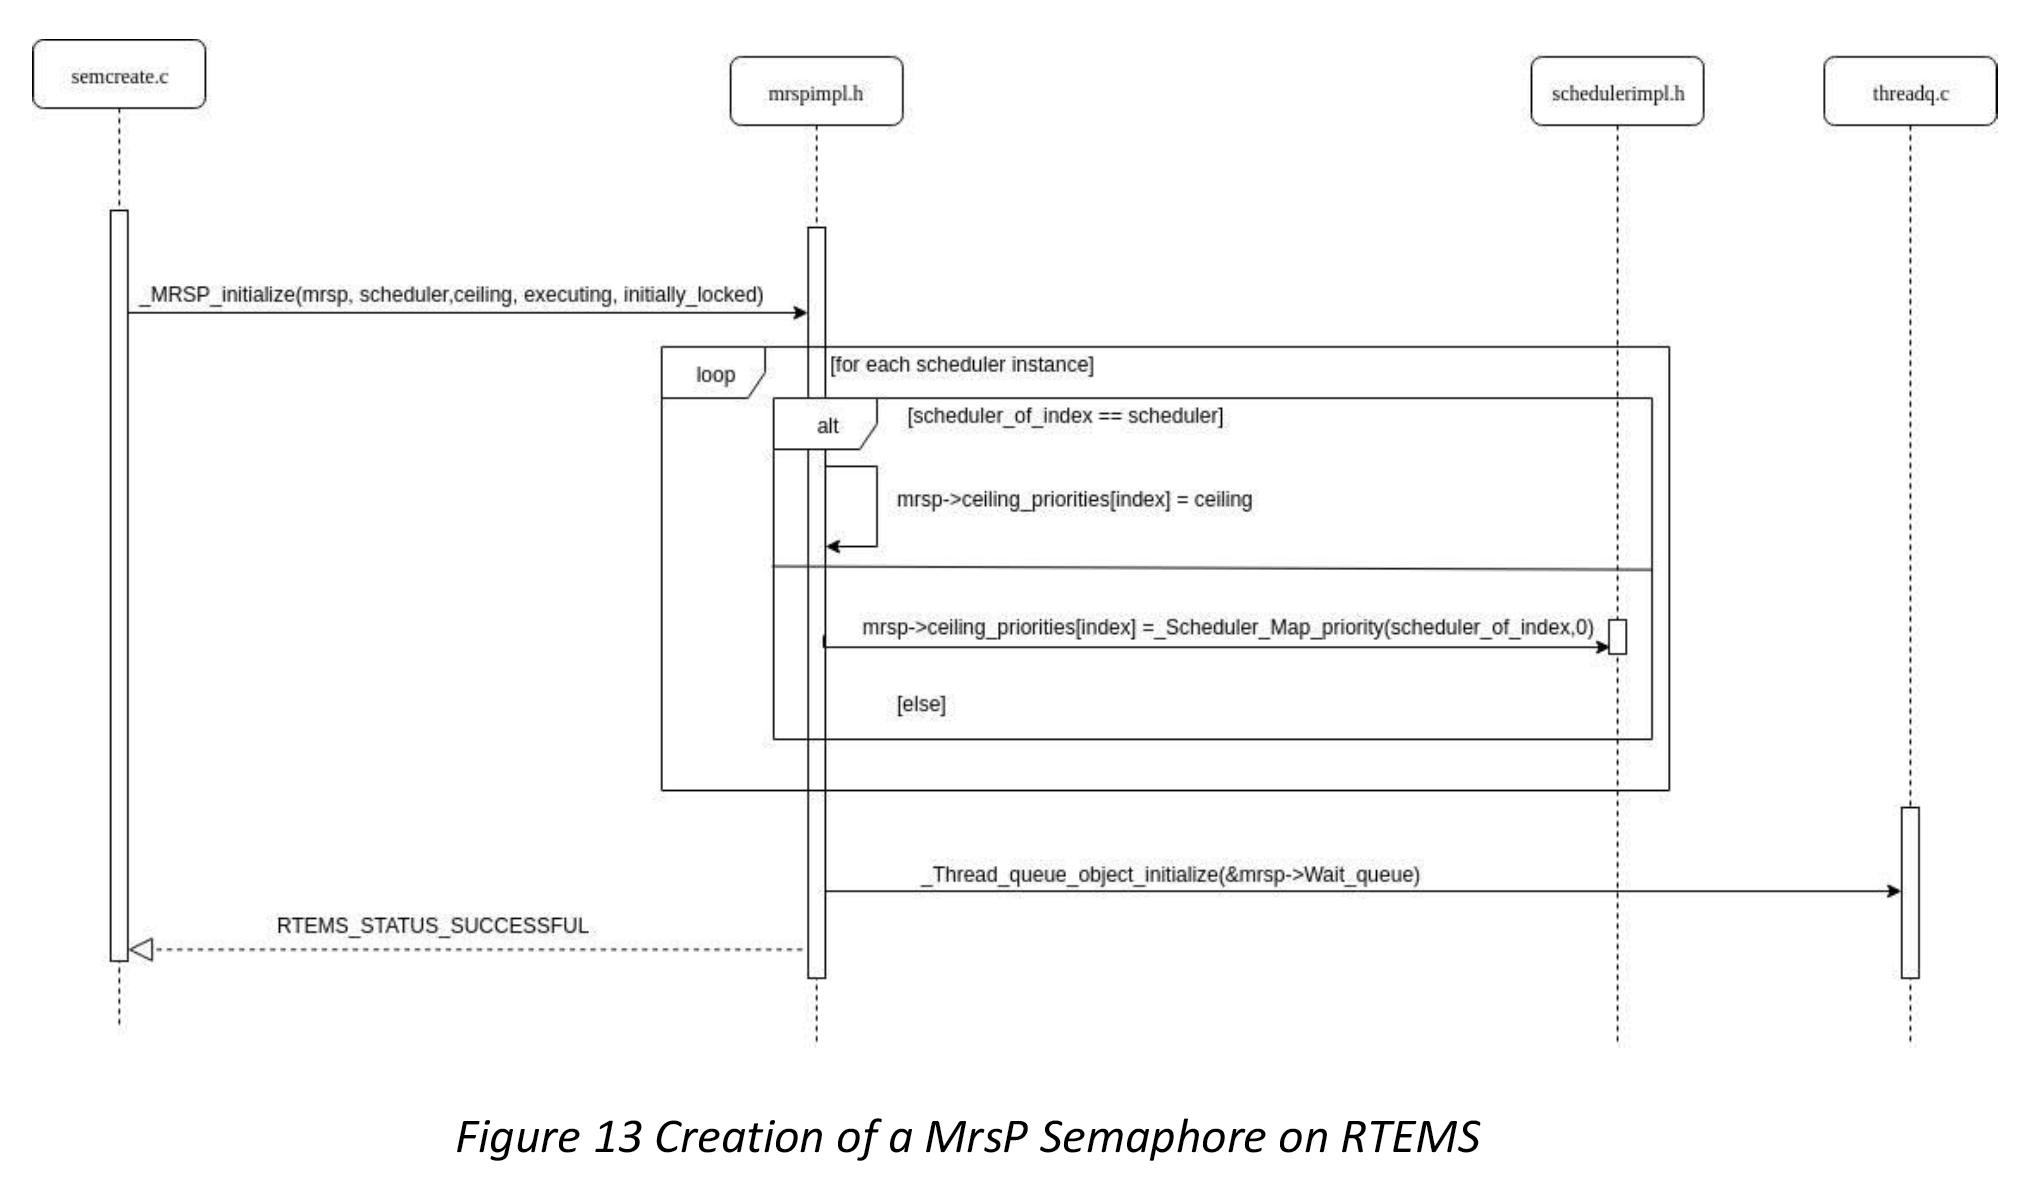
\includegraphics[width=\textwidth]{../images/create-MrsP-semaphore-Gomes-2019.png}

(p42) \textbf{How MrsP semaphores are initialised!}

\begin{quotation}
``
The sticky level of a task,
when incremented to at least the value of 1,
grants that when the task is executing
in any scheduler instance other than its original one,
lower priority tasks may not execute on its host scheduler,
with the purpose of securing this property.
This feature is quite relevant,
according to the properties of MrsP,
mentioned on chapter 3,
where it is defined that under semaphores using MrsP,
lower priority tasks must be
prevented from executing on the host processor of the holder of the resource.
'' (p45)
\end{quotation}


\textbf{Worth figuring out how to emulate the sets in Section 6}

\subsubsection{Appendix 2}

The purpose of \verb"_Thread_queue_Path_acquire_critical" is described here.


\subsection{Relevant code}
